\documentclass[10pt,a4paper]{amsart}

\usepackage{amsmath}
\usepackage{physics}
\usepackage{listings}
\usepackage{graphicx}
\usepackage{hyperref}
\usepackage[toc,page]{appendix}

\usepackage{color}
\definecolor{deepgreen}{rgb}{0,0.5,0}
\definecolor{mygray}{rgb}{0.9,0.9,0.9}
\definecolor{orange}{rgb}{0.9,0.3,0}

\lstset{
	frame = single,
	language = Python,
	showstringspaces = false,
	tabsize = 2,
	otherkeywords = {self},
	keywordstyle = \color{blue},
	identifierstyle=\color{deepgreen},
 	stringstyle=\color{orange},
 	backgroundcolor=\color{mygray}
}

\title[Micro and Macrostates in Thermal Physics]{Micro- and Macrostates in Thermal Physics \\
	\hrulefill\fbox{FYS2160}\hrulefill}
	
\author[Winther-Larsen]{Sebastian G. Winther-Larsen\\
\href{https://github.com/gregwinther/FYS2160/}{\texttt{github.com/gregwinther}}}

\date{\today}

\begin{document}

\maketitle

\tableofcontents

\section{Introduction}
This is a brief study of micro- and macrostates in thermal phyics and statistical mechanics\footnote{I have come to realise that these two terms are somewhat interchangeable}. In statistical mechanics, a microstate is a specific microscopic configuration of a thermodynamic system that the system may occupy with a certain probability in the course of its thermal fluctuations. In contrast, the macrostate of a system refers to its macroscopic properties, such as its temperature, pressure, volume and density. Two models are introduced in this study; \emph{the Einstein crystal}, which could respresent a silicone crystal, and the \emph{spin system}, which could represent a system of magnetic dipoles

\section{The Einstein Crystal}

\subsection{Theoretical background}
In a real crystal, individual atoms oscillate around an equilibrium posistion while interacting mostly with its nearest neighbors. A simplified model for such a system can be represented by a harmonic oscillator potential in three dimensions
\begin{equation}
U_i(\vb{r}_i)=\frac{1}{2}k_x(x_i-x_{i,eq})^2+\frac{1}{2}k_y(y_i-y_{i,eq})^2+\frac{1}{2}k_z(z_i-z_{i,eq})^2
\end{equation} 
From quantum mechanics, we know that the energy of a harmonic oscillator is
\begin{equation}
\epsilon_i=n_i\Delta \epsilon
\end{equation}
where $n_i$ is an integer describing the state of oscillator $i$. The entire system of $N$ such (non-interacting) oscillators will have total energy
\begin{equation}
\label{eq:totalU}
U=\sum_{i=1}^N \epsilon n_i
\end{equation}
For simplicity the energy is measured in units of $\epsilon$.
\begin{equation}
\label{eq:totalU2}
q = \frac{U}{\epsilon}=\sum_{i=1} n_i
\end{equation}
This is equivalent to equation \ref{eq:totalU}, but implies that a specific system will have constant total energy, yet the energy distribution may change.

A microstate of the Einstein crystal is described by the numbers $n_i$ for each oscillator
\begin{equation}
\{n_1,n_2,\dots,n_N\}
\end{equation}
For example, for a system with $N=4$ and $q=4$, a possible microstate is $\{1,0,2,1\}$.

\subsection{Simple microstates}
In a system with $N=3$ and $q=3$ there are ten possible microstates
\begin{align*}
&\{0,0,3\},\{3,0,0\},\{3,0,0\},\{0,1,2\},\{1,0,2\},\\
&\{1,2,0\},\{2,1,0\},\{2,0,1\},\{2,1,0\},\{1,1,1\}
\end{align*}
For an easy case like this it is relatively easy to write out all the different microstates. When the system is bigger, with higher $N$, a human may not be up for the task.

The general formula for computing the number of microstates for $N$ oscillators with $q$ units of energy is
\begin{equation}
\label{eq:binom}
\Omega(N,q)=\binom{q+N-1}{q}=\frac{(q+N-1)!}{q!(N-1)!}
\end{equation} 
Plugging in for $N=3$ and $q=3$ indeed yields the expected result
\begin{equation*}
\Omega(3,3)=\binom{3+3-1}{3}=\binom{5}{3}=\frac{5!}{3!2!}=\frac{5\cdot4}{2}=10
\end{equation*}

\subsection{Two subsystems in thermal contact}
Consider two initially isolated subsystems, system $A$ with $N_A=2$ oscillators and energy $q_A=5$; and system $B$ with $N_B=2$ oscillators and energy $q_B=1$. Subsystem $A$ has the following six possible microstates 
\begin{equation}
\{0,5\},\{1,4\},\{2,3\},\{3,2\},\{4,1\},\{5,0\}
\end{equation} 
and subsystem $B$ will have the following two microstates
\begin{equation}
\{0,1\},\{1,0\}
\end{equation}
All the microstates from one of the subsystems can be combined with any from the othes system giving a total number of $6\cdot2=12$ possible microstates.

Now, let the two subsystems be put in thermal contact. This means that they can exchange energy, but that the number of particles and volume of each subsystem does not change. The total energy ($q=q_A+q_B=6$) can be distributed between the two subsystems. The possible values of $q_k=q-q_{k^c}$ where $k \in \{A,B\}$. $k^c$ is the complement of $k$, whatever $k$ is not. It follows that the possible energy values must be $q_k \in [0,q]=[0,6]$.

We call a state with a given $q_A$ for a \emph{macrostate} of the combined system. This means that there are a total of seven macrostates in the system, listed in table \ref{tab:einsteinmacro}

\begin{table}[h]
\caption{Macrostates and mulitpicities of a system with two Einstein crystals}
\begin{tabular}{rrrrr} \hline
 $q_A$ & $\Omega_A$ & $q_B$ & $\Omega_B$ & $\Omega_{tot}$ \\ \hline
    0  &  1 &  6  &  7   &   7 \\
    1  &  2 &  5  &  6   &  12 \\
    2  &  3 &  4  &  5   &  15 \\
    3  &  4 &  3  &  4   &  16 \\
    4  &  5 &  2  &  3   &  15 \\
    5  &  6 &  1  &  2   &  12 \\
    6  &  7 &  0  &  1   &   7 \\ \hline
       &    &     & Sum: &  84 \\ \hline  
\end{tabular}
\label{tab:einsteinmacro}
\end{table}
These values have been calculated using the binomial coefficient in equation \ref{eq:binom}. The full number of microstates for a given macrostate $q_A$ are given in the last column as the total multiplicity $\Omega_{tot}=\Omega_A\Omega_B$.

The following source code listing provides a way to compute the same numbers with a class in Python.

\lstinputlisting[firstline=4, lastline=28]{einsteincrystals.py}

An object of this class defines a system consisting of two subsystems, $A$ and $B$. To get information about the states and multiplicity of the system I have written the following method\footnote{I am uncertain what names to use: object or class instance; and method or function. My sincere apologies to the reader if some other words than than the ones I have chosen are the norm for Python.}. This method displays information about smaller systems quite well.

\lstinputlisting[firstline=31, lastline=43]{einsteincrystals.py}

To compute probability of every state and to plot det probability density function I have writting this next method method which computes the probabilities for the macrostates $q_A$. The probability are computed by dividing all possible microstates for a given macrostate by every possible micorstate.
\begin{equation}
p(q_A)=\frac{\Omega_{i,tot}}{\sum\Omega_{i,tot}}
\end{equation}

\lstinputlisting[firstline=46, lastline=61]{einsteincrystals.py}
The method prints to terminal the probabilities that are given in table \ref{tab:einsteinprobs}.
\begin{table}[h]
\caption{Probabilities of the macrostates for two Einsten crystals where $q=6$ and $N_A=N_B=2$}
\begin{tabular}{cc} \hline
 $q_A$ & $P(q_A)$ \\ \hline
 0 & 0.0833 \\
 1 & 0.1429 \\
 2 & 0.1786 \\
 3 & 0.1905 \\
 4 & 0.1786 \\
 5 & 0.1429 \\
 6 & 0.0833 \\ \hline
 Sum: & 1.0 \\ \hline
\end{tabular}
\label{tab:einsteinprobs}
\end{table}

The maximium number of microstates before the two crystals came in thermal contact was only $\sum\Omega_{i,tot}=12$. For the interconnected system, the number of allows microstates have risen dramatically to $\sum\Omega_{i,tot}=84$. Another aspect to draw attention to is that the highest number of possible microstates for a givin macrostate is highest when the energy in the crystals, $q_A$ and $q_b$ are similar. This is clear from looking at table \ref{tab:einsteinmacro}. It would be intersting to see if the same holds true for an even larger system. Figure \ref{fig:EinsteinPDF} shows the an approximation of a probability density function for the two crystals when the parameters are increased to $q=100$ and $N_A=N_B=50$. The tendency is very clear, as we see the graph forms a characteristic bell curve with a peak at $q_A=50$, where the energy of the two crystals are most similar. The probability for this exact macrostate is $p(q_A=50) \approx 5.6\%$.

\begin{figure}[h]
  \centering
  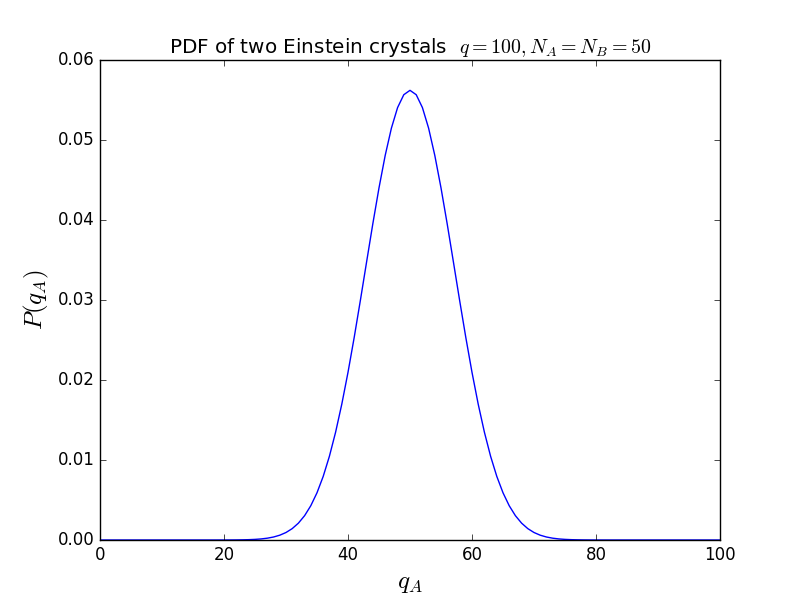
\includegraphics[width=0.9\linewidth]{EinsteinPDF.png}
  \caption{Probability density function for two interconnected Einstein crystals with $q=100$ and $N_A=N_B=50$}
  \label{fig:EinsteinPDF}
\end{figure}

\subsection{Thermodynamic properties}
Equation \ref{eq:binom} gives us the multiplicity of a system as a binomial coefficient
\begin{equation*}
\Omega(N,q)=\binom{q+N-1}{q}=\frac{(q+N-1)!}{q!(N-1)!}
\end{equation*}
Using Stirlings's approximation, $\ln x!=x\ln x-x$, this expression can be simplified for large $N$. First of all the exact formula can be simplified
\begin{equation}
\frac{(q+N-1)!}{q!(N-1)!} \approx \frac{(q+N)!}{q!N!}
\end{equation}
Now we take the natural logarithm and apply Stirling's approximation
\begin{align}
\ln \Omega &\approx \ln \left(\frac{(q+N)!}{q!N!}\right) = \ln (1+n)! - \ln q! - \ln N! \\
& \approx (q+N)\ln (q+N)-(q+N) - q \ln q +q - N \ln N +N \\
&= (q+N) \ln (q+N) - q \ln q - N \ln N \\
&= (q+N) \ln q(1+\frac{N}{q}) - q \ln q - N \ln N \\                                                                                                                                                                                                                                                                                                                                                                                                       
&= (q+N) (\ln q + \ln(1+\frac{N}{q})) - q \ln q - N \ln N                                                                                                                                                                                                                                                                                                                                                                                                       
\end{align}
A Taylor expansion will reveal that $\ln (1+x) \approx x$. Then we have
\begin{align*}
\ln \Omega &\approx (q+N) (\ln q + \frac{N}{q}) - q \ln q - N \ln N\\
&= q\ln q + N + N \ln q + \frac{N^2}{q} - q\ln q - N\ln N \\
&= N \ln \left(\frac{q}{N}\right) +N + \frac{N^2}{q} 
\end{align*}
Assuming $N/q << 1$, then $N^2/q$ will quickly approach zeros, and we are left with a very neat expression for the natural logarithm of the mulitiplicity
\begin{equation}
\label{eq:lnmulti}
\ln \Omega (N,q) \approx N(\ln (q/N) +1)
\end{equation}

From equation \ref{eq:lnmulti} one can see that the multiplicity of a large Einstein solid must be 
\begin{equation}
\label{eq:largemulti}
\Omega (N,q) \approx e^{N \ln (q/N)}e^= \left(\frac{eq}{N}\right)^N
\end{equation}

For a variety of systems, particles and energy tend to rearrange themselves until the multiplicity is at or very near its maximum value. The fact that the multiplicity tends to increase is a simple way to state the \emph{second law of thermodynamics}.

Since multiplicities are very large numbers, one usually deals with the natural logarithm to the multiplicity instead. This was the reason for the rather large algebraic exercise war performed above. For historical reasons, one also multiply by a factor of Boltzmann's constant. This provides a quantity called the \emph{entropy}.
\begin{equation}
\label{eq:entropy}
S \equiv k \ln \Omega
\end{equation} 
For a large Einsten crystal the entropy must be
\begin{equation}
\label{eq:einsteinentropy}
S=k \ln (eq/N)^N = Nk[\ln (q/N) + 1]
\end{equation}

One nice property of entropy is that the total entropy of a system of several subsystemsis the sum of the entropy of the subsystems. For a two-part system a quick proof will be something like this
\begin{equation}
S_{tot}=k \ln \Omega_{tot} = k \ln (\Omega_A\Omega_B) = k \ln \Omega_A + k \ln \Omega_B = S_A + S_B
\end{equation}

Consider a thermal equilibrium of two Einstein crystals in thermal contact. At equiliribrium the entropy, as a function of energy, of the two crystals must be at maximum. In other words, algebraically speaking
\begin{equation}
\frac{\partial S_A}{\partial U_A} + \frac{\partial S_B}{\partial U_B} = 0
\end{equation}
where $U_k= \epsilon q_K$ (the energy of each particle times the unit of energy\footnote{This follows from equation \ref{eq:totalU} and \ref{eq:totalU2}}). 

The definition of \emph{temperature} of a system is the reciprocal of the slope of its entropy vs energy graphs. Again, algebraically speaking
\begin{equation}
T \equiv \left(\frac{\partial S}{\partial U} \right)^{-1}
\end{equation}
By expanding upon the expression for entropy of an Einstein crystal (equation \ref{eq:einsteinentropy})
\begin{equation}
S= Nk[\ln (q/N) + 1]
= Nk \ln U -Nk \ln (\epsilon N) + Nk
\end{equation}
one will find the temperature of the Einstein crystal to be
\begin{equation}
T = \left(\frac{\partial S}{\partial U} \right)^{-1}
= \left(\frac{Nk}{U} \right)^{-1} = \frac{U}{Nk} 
\end{equation}

\section{The Spin System}
The spin system is different from a system of Einstein crystals, but can be addressed in a somewhat similar approach. For a paramegnetic system with binary spins, each particle can be in two possible states $S=+1$ or $S=-1$. Alternatively, one can call theses states "spin up" and "spin down" states, borrowing terminology from quantum mechaninics\footnote{This quickly becomes a study of a spin-$1/2$ particle system}. The energy of such a dipole depends on its orientation relative to an external magnetic field $B$. The simplest system we can consider consists of $N$ independent dipoles/spins, $S_i$. 

If we define $N_{\uparrow}$ to be the number of dipoles that point up, and $N_{\downarrow}$ to be the number of dipoles that point down, the total number of dipoles is $N=N_{\uparrow}+N_{\downarrow}$. For a system of a given $N$, there will be one macrostate for each possible value of $N_{\uparrow}$ from $0$ to $N$. It is easy to see that the number of different systems is governed by combinatorical mathematics and the multiplicity of any given macrostate is therefore given by the binomial coefficient
\begin{equation}
\Omega(N_{\uparrow}) = \binom{N}{N_{\uparrow}}=\frac{N!}{N_{\uparrow}!(N-N_{\uparrow})!}=\frac{N!}{N_{\uparrow}!N_{\downarrow}!}
\end{equation}
which is another way of saying; "how many different systems of a given number of spin up can I have?". I have supplied an attempt at a derivation of the binomial coefficient in appendix \ref{app:binom}, for the keen reader.

For the sake of symmetry, the energy levels of a single dipole in an ideal two-state paramagnet are $-\mu B$ for spin up and $\mu B$ for spin down. The total energy of the system is
\begin{equation}
U = \mu B(N_{\downarrow}-N_{\uparrow})
\end{equation}
denoting the net spin by $\nu$, it is given by the relation $2\nu = N_{\uparrow}-N_{\downarrow}$. It can be beneficial to write the total energy as a function of the net spin:
\begin{equation}
U = -2\mu B \nu
\end{equation} 

By rewriting the number of spin up dipoles
\begin{equation}
N_{\uparrow}=N-N_{\downarrow}=\frac{N}{2}+\frac{N}{2}+N_{\downarrow}
=\frac{N}{2}+\frac{N_{\uparrow}}{2}+\frac{N_{\downarrow}}{2}-\frac{2N_{\downarrow}}{2}=\frac{N}{2}+\frac{N_{\uparrow}-N_{\downarrow}}{2}=\frac{N}{2}+\nu
\end{equation}
and similarly for spin down dipoles
\begin{equation}
N_{\downarrow}=N-N_{\uparrow}=\frac{N}{2}+\frac{N}{2}+N_{\downarrow}
=\frac{N}{2}+\frac{N_{\uparrow}}{2}+\frac{N_{\downarrow}}{2}-\frac{2N_{\uparrow}}{2}=\frac{N}{2}-\frac{N_{\uparrow}-N_{\downarrow}}{2}=\frac{N}{2}-\nu
\end{equation}
This in turn allows one to rewrite the multiplicity as a function of the net spin
\begin{equation}
\Omega (N,\nu) = \frac{N!}{\left(\frac{N}{2} +\nu\right)!\left(\frac{N}{2} -\nu\right)!}
\end{equation}

\begin{appendices}
\section{Deriving the binomial coefficient}
\label{app:binom}
This ouline may not be rigorous enough to satisfy a mathematician, but it serves its purpose, in the true spirit of a physicist.

Say we have an $n$ element set and want to make ordered lists of length $k$ from this set. There will be $n$ ways to pick the first element, $n-1$ ways to pick the second, and $n-k$ ways to pick the $k$th element. Alternatively, there are
\begin{equation}
n(n-1)\dots(n-k)=\frac{n!}{(n-k)!}
\end{equation}
such sequences.
This is all nice and dandy, but we are in reality dealing with \emph{unordered} lists. This means that we want to identify the $k!$ permutations of its elements, each of which was counted seperately above as the same list. The fix is simple - Divide by $k!$:
\begin{equation}
\frac{\frac{n!}{(n-k)!}}{k!}=\frac{n!}{k!(n-k)!}
\end{equation}
This is the binomial coefficient. Q.E.D.
\end{appendices}

\end{document}
